\documentclass[a4paper]{scrartcl}

\usepackage[T1]{fontenc}
\usepackage[utf8]{inputenc}
\usepackage[ngerman]{babel}

\usepackage{hyperref}

\usepackage{wrapfig}
\usepackage{caption}
\usepackage{graphicx}
\usepackage{xcolor}
\usepackage{courier}
\usepackage{listings}
\usepackage{pdfpages}
\usepackage{float}

\usepackage{microtype}

\usepackage[backend=bibtex]{biblatex} 
\addbibresource{dynasmgb.bib}

\lstdefinelanguage
   [x64]{Assembler}     % add a "x64" dialect of Assembler
   [x86masm]{Assembler} % based on the "x86masm" dialect
   % with these extra keywords:
   {morekeywords={CDQE,CQO,CMPSQ,CMPXCHG16B,JRCXZ,LODSQ,MOVSXD, %
                  POPFQ,PUSHFQ,SCASQ,STOSQ,IRETQ,RDTSCP,SWAPGS, %
                  LD, LDH, JR, CP, CALL,
                  rax,rdx,rcx,rbx,rsi,rdi,rsp,rbp, %
                  r8,r8d,r8w,r8b,r9,r9d,r9w,r9b}} % etc.

\lstset{ %
  language=[x64]Assembler,       % the language of the code
  basicstyle=\ttfamily,       % the size of the fonts that are used for the code
  %numbers=left,                   % where to put the line-numbers
  %numberstyle=\tiny\color{gray},  % the style that is used for the line-numbers
  %stepnumber=1,                   % the step between two line-numbers. If it's 1, each line 
                                  % will be numbered
  %numbersep=5pt,                  % how far the line-numbers are from the code
  backgroundcolor=\color{white},  % choose the background color. You must add \usepackage{color}
  showspaces=false,               % show spaces adding particular underscores
  showstringspaces=false,         % underline spaces within strings
  showtabs=false,                 % show tabs within strings adding particular underscores
  frame=single,                   % adds a frame around the code
  %rulecolor=\color{black},        % if not set, the frame-color may be changed on line-breaks within not-black text (e.g. commens (green here))
  tabsize=4,                      % sets default tabsize to 2 spaces
  captionpos=b,                   % sets the caption-position to bottom
  breaklines=true,                % sets automatic line breaking
  breakatwhitespace=false,        % sets if automatic breaks should only happen at whitespace
  title=\lstname,                 % show the filename of files included with \lstinputlisting;
                                  % also try caption instead of title
%  keywordstyle=\color{blue},          % keyword style
  commentstyle=\color{green},       % comment style
  stringstyle=\color{mauve},         % string literal style
  escapeinside={\%*}{*)},            % if you want to add a comment within your code
  morekeywords={*,...},               % if you want to add more keywords to the set
%  
  belowskip=0em,
  aboveskip=2em
}

% Hurenkinder und Schusterjungen verhindern
\clubpenalty10000
\widowpenalty10000
\displaywidowpenalty=10000

\title{Entwicklung eines Gameboy-Emulators}
\author{Thomas Witte}
\date{\today}

\begin{document}
\maketitle

\section{Motivation / Emulation}

Der 1989 von Nintendo hergestellte Gameboy ist mit über 100 Millionen verkauften Einheiten eine der erfolgreichsten Spielekonsolen überhaupt.

\begin{wrapfigure}{r}{0.4\textwidth}
%\begin{figure}[H]
\centering
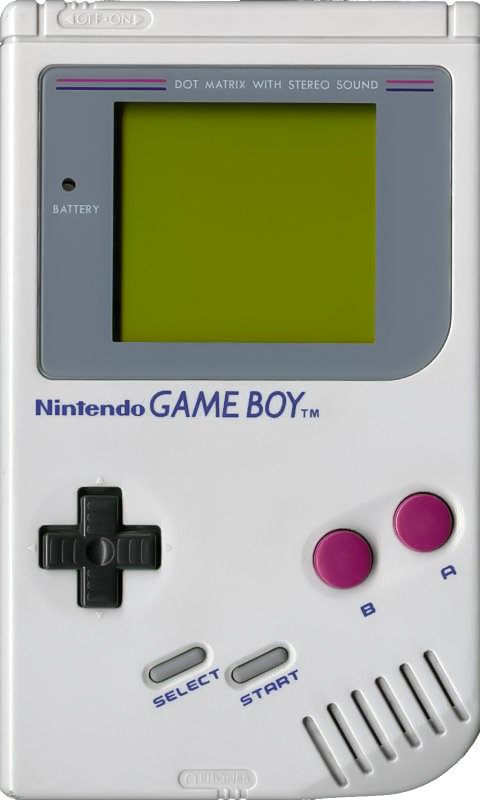
\includegraphics[width=0.9\linewidth]{img/Gameboy.jpg}
\caption{Gameboy der ersten Generation.}
\label{img:gameboy}
%\end{figure}
\end{wrapfigure}

Da die meisten für den Gameboy erschienenen Spiele nur in binärer Form als ROM-Abbild vorliegen, ist eine Portierung auf aktuelle Systeme ausgeschlossen. Eine Alternative bietet die Emulation der Gameboy-Architektur: es wird eine möglichst exakt dem Gameboy gleichende Laufzeitumgebung bereitgestellt, die in der Lage ist, das unmodifizierte Programm auszuführen. Dazu müssen neben der CPU auch sämtliche anderen Schnittstellen (Ein-/Ausgabe, Speicher, etc.) bereitgestellt werden.

Aufgrund der inkompatiblen Prozessorarchitekturen kann die Instruktionsfolge des emulierten Programms nicht direkt ausgeführt werden: entweder wird sie Instruktion für Instruktion interpretiert, also der Fetch-Execute-Cycle in Software durchgeführt, oder in kompatible Instruktionen übersetzt. Das zweite Verfahren -- oft „dynarec“ oder „jit-compiler“ genannt -- wird in vielen Emulatoren aufgrund der potentiell höheren Geschwindigkeit verwendet \cite{pcsx2_introduction}.

Die Übersetzung der Instruktionen geschieht meist dynamisch zur Laufzeit, da durch statische Analyse nur schwer -- zB durch verfolgen aller möglichen Ausführungspfade ab einem bekannten Einsprungpunkt -- zwischen Daten und Programmtext unterschieden werden kann. Selbstmodifizierender Code und das Anspringen von zur Laufzeit berechneten Adressen macht bei statischer Übersetzung zusätzlich häufig eine Rückfall auf Interpretation oder dynamische Übersetzung zur Laufzeit notwendig \cite{nes_recompiler}.

Der im Zuge des Projekts entstandene Emulator „dynasmgb“ führt daher eine dynamische Übersetzung der Prozessorinstruktionen aus. Sämtliche anderen Schnittstellen (Grafik, Sound, Speicher) werden jedoch weiterhin vollständig in Software umgesetzt.

%Warum ist Emulation notwendig
%Was muss emuliert werden
%Interpretation vs jit vs aot
%existierende Gameboy Emulatoren
\section{Gameboy Architektur}

Die folgenden Abschnitte fassen Aufbau und Funktionsweise des klassischen Gameboys zusammen. Auf die Unterschiede zum Gameboy Color und Super Gameboy wird nicht eingegangen. Details finden sich in \cite{cpu_manual}\cite{gb_programming_manual}\cite{pandocs}.

\subsection{Hardware}

Herzstück des Gameboy ist ein leicht modifizierter Z80 Prozessor, der mit 4,2MHz getaktet ist. Der Registersatz besteht -- ähnlich auch einem Intel 8080 -- aus 7 8bit Registern, einem Flagregister (Zero, Carry, Halfcarry, Subtract) sowie zweier 16bit Register (SP und PC). Die 8bit Register können durch bestimmte 16bit Instruktionen jeweils paarweise als 16bit Register genutzt werden.

Der Gameboy kann auf insgesamt 16kB internen Arbeitsspeicher zugreifen. Dabei sind 8kB dieses Speichers als Tile-RAM für Grafiken zweckgebunden. Der Memory Bank Controller (MBC) bestimmter Spiele kann bis zu 128kB zusätzlichen RAM innerhalb der Cartridge adressieren (16 Bänke à 8kB).

Das Spiel wird direkt aus dem ROM der Spiel-Cartridges gestartet. Über MBCs können dabei maximal 4MB (256 Bänke à 16kB) adressiert werden.

Als Display kommt ein Graustufen-LCD zum Einsatz. Es kann 4 Grautöne darstellen und besitzt eine Auflösung von $160 \times 144$ Pixel bei 60Hz. Die Pixel des Displays können dabei nicht einzeln angesprochen werden, sondern nur in $8 \times 8$ Pixel großen Kacheln (Tiles).

Dabei kann gleichzeitig eine Hintergrundkarte, eine Vordergrundkarte und bis zu 40 Sprites angezeigt werden.

Die Soundausgabe erfolgt über einen integrierten Lautsprecher oder den Kopfhörerausgang in Stereo. Der Gameboy bietet dazu vier Soundkanäle, die Rechteckschwingungen, Rauschen oder Wave-Samples erzeugen bzw. abspielen können.

Zur Eingabe stehen insgesamt acht Knöpfe zur Verfügung (vier Richtungstasten, A, B, Select und Start). Alternativ können Daten über eine serielle Schnittstelle gesendet oder empfangen werden.
%Prozessor, Speicher, Takt, Display, Registersatz, IO ...
\subsection{Befehlssatz}

Der Befehlssatz umfasst insgesamt 500 verschiedene Befehle variabler Instruktionslänge (1-3 Bytes). 244 Befehle nutzen das erste Byte für den Opcode und maximal zwei Bytes für Argumente. Die restlichen 256 Befehle werden durch das Präfixbyte 0xCB eingeleitet und besitzen somit einen 2Byte-Opcode und keine weiteren Argumente.

Die Ausführungszeit der Befehle beträgt jeweils zwischen 4 und 24 Taktzyklen. Damit beträgt der maximale Befehlsdurchsatz 1MOps/s.

Eine Übersicht sämtlicher Befehle befindet sich unter \cite{gameboy_opcodes}, sowie im Anhang.

%Bild im Anhang, wichtige Instruktionen
\subsection{Interrupts}

Der Gameboy stellt insgesamt fünf verschiedene Interrupts zur Verfügung:

\begin{description}
\item[VBLANK]
Der VBLANK-Interrupt wird nach jedem dargestellten Bild dargestellt und markiert den Beginn der VBLANK-Phase in der für 4560 Taktzyklen frei auf den Videospeicher zugegriffen werden kann.
\item[STAT]
Das STAT-Register (Speicheradresse 0xFF41) wechselt mit jeder dargestellten Bildzeile zwischen drei Zuständen und während der VBLANK-Phase auf einen vierten. Der STAT-Interrupt kann bei einem Wechsel dieser Zustände ausgelöst werden. Welche Zustandsübergänge betroffen sind, kann ausgewählt werden.
\item[Timer]
Der Timer-Interrupt wird bei einem Überlauf des Timer-Registers (0xFF05) ausgelöst. Die Rate mit der das Timer-Register inkrementiert wird ist dabei auswählbar, sodass der Timer-Interrupt mit einer wählbaren Rate von 16Hz, 64Hz, 256Hz oder 1kHz auftritt.
\item[Serial]
Der Serial Transfer-Interrupt wird beim Abschluss eines seriellen Transfers ausgelöst.
\item[Joypad]
Bei jedem Tastendruck eines der acht Knöpfe wird der Joypad-Interrupt ausgelöst.
\end{description}

Tritt ein Interrupt auf, so wird er anhängig und ein Bit im Interrupt Flag-Register (0xFF0F) gesetzt.
Über das Interrupt Enable Register (0xFFFF) kann ausgewählt werden, welche Interrupts aktiv sind.
Das Interrupt Master Enable-Flag kann zusätzlich alle Interrupts abschalten. Es kann durch die Instruktionen DI (Disable Interrupts), EI (Enable Interrupts) oder RETI (Return from Interrupt) manipuliert werden.

Ist ein Interrupt anhängig, das entsprechende Bit im Interrupt Enable Register gesetzt und das Interrupt Master Enable-Flag gesetzt wird eine Handlerfunktion mit fester Startadresse zwischen 0x40 (VBLANK) und 0x60 (Joypad) aufgerufen und mittels des Interrupt Master Enable weitere Interrupts während der Behandlung unterbunden.
%Interrupts, Startadressen, ...
\subsection{Adressraum}

\subsubsection{Memory Map}

Der adressierbare Adressraum des Gameboys beträgt 64kB. In die unteren 32kB (0x0 - 0x7FFF) werden zwei Rombänke à 16kB gleichzeitig eingeblendet. Der Wechsel zwischen den Rombänken geschieht durch den MBC innerhalb der Cartridge. Alle verfügbaren MBCs lösen einen Wechsel der oberen Rombank durch Schreibzugriffe auf bestimmte Adressen im ROM aus.

\begin{figure}[H]
\centering
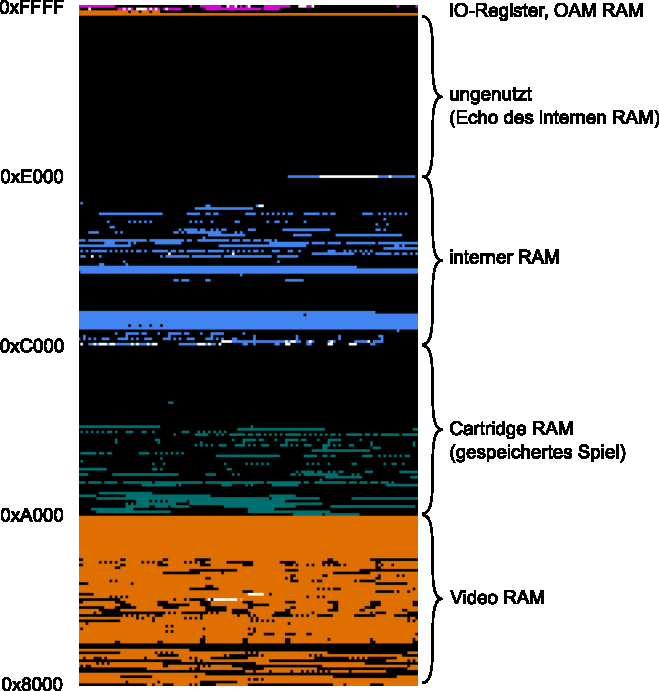
\includegraphics[width=0.75\linewidth]{img/mmap.pdf}
\caption{Visualisierung der oberen 32kB des Adressraums (Pokémon Blaue Edition)}
\label{img:sound}
\end{figure}

Die Adressen zwischen 0x8000 und 0x9FFF bilden den Video-RAM. Er enthält $8 \times 8$ Pixel große Kacheln zu je 16 Byte, sowie Vordergrund und Hintergrund Tile Maps.

Zwischen 0xA000 und 0xBFFF wird der Cartridge RAM eingeblendet. Je nach MBC lassen sich eventuell mehrere Bänke tauschen. Dieser Speicher ist in einigen Spielcartridges durch eine Batterie versorgt und kann damit auch bei ausgeschaltetem Gameboy einen Spielstand halten.

Es folgen 8kB interner RAM (0xC000 - 0xDFFF), der fast vollständig ein zweites Mal im Adressbereich 0xE000 - 0xFDFF gespiegelt wird. Diese Adressen werden jedoch typischerweise nicht verwendet.

Die Adressen 0xFE00 bis 0xFE9F enthalten den OAM Speicher. Er enthält die Position, anzuzeigende Grafik, verwendete Graustufenpalette und Flags aller 40 Sprites. Per DMA-Transfer kann der OAM Speicher nebenläufig überschrieben werden.

Über den Adressbereich 0xFF00 bis 0xFF7F wird der Hardware IO gesteuert. Er enthält Register zur Kontrolle von Timern, Seriellen Übertragungen, DMA-Transfers, Soundausgabe und des anzuzeigenden Mapbereichs.

Im Anschluss befinden sich weitere 127 Byte Arbeitsspeicher (0xFF80 - 0xFFFE), die jederzeit les- und schreibbar sind. Da während eines DMA-Transfers der gesamte sonstige Speicher weder gelesen noch geschrieben werden kann, muss während eines solchen Transfers in diesen Speicherbereich gesprungen werden.

Das Interrupt Enable Register belegt die höchste Adresse 0xFFFF.

\subsubsection{Startadressen}

Die Ausführung des Programms beginnt an Adresse 0x100. Die Handlerfunktionen mit den Startadressen zwischen 0x00 und 0x60 werden durch Restarts und Interrupts angesprungen. 

\subsubsection{ROM-Header}

Die Rom-Adressen 0x104 bis 0x14F sind durch den ROM-Header belegt. Er enthält eine Grafik, die das Nintendo-Logo zeigt (0x104 bis 0x133). Diese wird auf realen Konsolen beim Start angezeigt und verglichen. Stimmt sie nicht exakt überein, startet der Gameboy das Spiel nicht. Die weiteren Bytes enthalten Spieltitel, Hersteller, Flags die anzeigen, ob das Spiel spezielle Funktionen für Gameboy Color oder Super Gameboy enthält, sowie Informationen über den verbauten MBC und die Anzahl der auf der Cartridge vorhandenen RAM- und ROM-Bänke.
%Layout, MBCs, Startsequenz, Memory-Banking, ROM-Header, Spiele speichern
\subsection{Grafik}

Die Pixel des Gameboydisplays können nicht einzeln angesprochen werden, sondern es werden immer ganze Kacheln von jeweils $8 \times 8$ Pixel Größe angezeigt. Neben einer Vordergrund- und Hintergrundkarte (WIN und BG genannt) die die Indizes der anzuzeigenden Kacheln enthalten, können bis zu 40 Sprites frei auf dem Display positioniert werden.

Das Bild wird zeilenweise von oben nach unten aufgebaut. Über das Register LY (0xFF44) kann die derzeit bearbeitete Zeile ausgelesen werden und über das STAT Register (0xFF41) ob derzeit ein Zugriff auf den Grafikspeicher möglich ist.

Die Größe der Vordergrund- und Hintergrundkarte beträgt 32 auf 32 Kacheln, sodass immer nur ein Ausschnitt auf dem Display sichtbar ist. Über die Register SCX (Scroll X, 0xFF43), SCY (Scroll Y, 0xFF42), WX (Window X, 0xFF4B) und WY (Window Y, 0xFF4A) kann der anzuzeigende Bereich gewählt werden. Durch Änderung des sichtbaren Bereichs während des Bildaufbaus können Welleneffekte auf dem Display erzeugt werden.

\begin{figure}[htbp]
\centering
\includegraphics[width=\linewidth]{img/bg_tiles}
\caption{Bestimmung des Helligkeitswerts eines Hintergrundpixels}
\label{img:bg_tiles}
\end{figure}

Abbildung~\ref{img:bg_tiles} zeigt exemplarisch, wie die Farbe eines Hintergrundpixels zustande kommt: zunächst werden für die aktuell gezeichnete Bildzeile die Kachelindizes aus der Background Tile Map bestimmt; diese liegt wählbar entweder ab 0x9800 oder 0x9C00. Über diesen Index wird die Tile Data Table ab 0x8000 oder 0x8800 indiziert. Der Helligkeitswert des $x$-ten Pixels der $y$-ten Kachelzeile kann dann aus dem $x$-ten Bit des $2 \cdot y$-ten und $2 \cdot y+1$-ten Bytes aufgebaut werden. Der Aufbau für ein Vordergrundpixel erfolgt analog.

Bei der Anzeige von Sprites kommt statt einer Tilemap, der OAM-Speicher zum Einsatz: Er enthält für jeden der 40 Sprites eine 4 Byte Struktur, die neben der Bildschrimposition den Kachelindex und einige Flags enthält. Über diese Flags kann der Sprite gespiegelt, hinter dem Hintergrund oder mit einer anderen Graustufenpalette angezeigt werden.
%Timing, Effekte, Speicher, DMA, Tilekodierung, Graustufenpaletten
\subsection{Audio}

Der Gameboy verfügt über vier Kanäle zur Klangerzeugung, die beliebig in die Stereo-Ausgabekanäle gemischt werden können.

Kanal 1 und 2 erzeugen Rechteckschwingungen mit wählbarer Frequenz, Duty-Cycle und linearer Hüllkurve (Abbildung~\ref{img:sound}). Kanal 1 kann zusätlich noch eine Frequenzänderung („Sweep“) eines Tons erzeugen.

\begin{figure}[htbp]
\centering
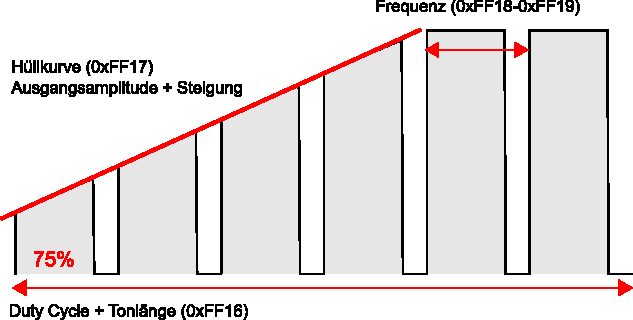
\includegraphics[width=0.9\linewidth]{img/sound}
\caption{Parameter für die Tonerzeugung auf Kanal 2}
\label{img:sound}
\end{figure}

Kanal 3 kann kann Wave-Samples abspielen. Der Wave-RAM aus dem diese gelesen werden ist auf 32 Samples à 4 Bit beschränkt.

Kanal 4 erzeugt weißes Rauschen. Dabei kann die Rauschcharakteristik beeinflusst werden um „weicheres“ oder „härteres“ Rauschen zu erzeugen.
%Timing, Effekte, Register
\section{Aufbau des jit-Übersetzers}

Für die Emulation der Gameboy Hardware auf herkömmlichen PCs (x86-64 Architektur) wurde ein just-in-time-kompilierender Emulationskern implementiert. Anstatt einzelne Instruktionen in einer Schleife zu dekodieren und interpretieren, wie bei einem interpretierenden Emulator, wird versucht ganze Blöcke, die gewöhnlich mit einer Sprunginstruktion (JP, JR, CALL, RST, RET, RETI) enden, zusammenzufassen. Mittels des Laufzeitassemblers „dynasm“ des Luajit Projekts \cite{dynasm_unofficial}\cite{dynasm} wird zum ersten Zeitpunkt, zu dem eine Speicheradresse angesprungen wird, dem Block entsprechende x86-Instruktionen erzeugt und ausgeführt.

Ein Ziel bei der Entwicklung war, möglichst die Statusflags (Carry, Halfcarry/Adjust und Zero) der Hostarchitektur für die emulierte Umgebung zu nutzen, anstatt diese zu emulieren. Dies ist in den meisten Fällen problemlos möglich, da sich die Z80-artige Gameboy CPU und die Intel 8080-Architektur, die größtenteils auch von modernen Prozessoren unterstützt wird sehr ähnlich sind. Da das Subtract-Flag des Gameboy keine direkte Entsprechung in der x86-64 Architektur besitzt muss es als einziges der Statusflags emuliert werden.

Sprünge werden nicht direkt ausgeführt, sondern stattdessen das Sprungziel gespeichert und die erzeugte Funktion mit RET verlassen. Dadurch kann die Laufzeitumgebung gegebenenfalls zunächst den Block am Sprungziel übersetzen und andere parallele Aufgaben ausführen. Diese umfassen die Interrupt, Grafik, Eingabe und DMA Emulation\footnote{Die Soundemulation läuft komplett asynchron in einem eigenen Thread und benötigt daher keine Unterbrechung des Programmablaufs.}.

Während der Übersetzung eines Programmblocks wird für jedes mögliche Ende über das der Block verlassen werden kann\footnote{Durch bedingte Sprünge können dies beliebig viele sein.}, die Anzahl der bis zu diesem Punkt benötigten Gameboy-Taktzyklen berechnet und diese Summe bei der Ausführung auf einen Instruktionszähler addiert. Mittels dieses Zählers können auf dem Gameboy zu bestimmten Zeitpunkten auftretende Ereignisse wie Timer- oder VBLANK-Interrupts trotz der höheren Geschwindigkeit der Hostplattform zeitlich genau ausgeführt werden. Da eventuell Routinen in den emulierten Programmen existieren, die auf eine feste Anzahl ausgeführter Instruktionen in einem bestimmten Zeitraum angewiesen sind, können nicht ohne Kompatibilitätsprobleme Timer des Hostsystems benutzt werden. Aufgrund der blockweisen Ausführung besteht jedoch auch bei dem hier vorgestellten Emulator das Problem, dass Interrupts oder Timer erst um einige Takte verspätet -- nach dem nächsten Sprung -- ausgeführt beziehungsweise aktualisiert werden.

Während der Ausführung übersetzter Programmblöcke wird der Registersatz des Gameboy direkt auf Register der x86-64 Architektur abgebildet. Am Ende eines Blocks muss dann der gesamte Gameboy-Registersatz, Prozessorflags und die Anzahl emulierter Taktzyklen gesichert werden (struct gb\_state). Tabelle~\ref{tab:register} stellt die Registernutzung während der Ausführung übersetzter Blöcke dar. Die für die 16 Bit Instruktionen des Gameboy nötigen kombinierten Register AF, BC, DE und HL werden bei Bedarf zunächst in einem temporären Register zusammengesetzt und nach der Instruktion wieder zurückgeschrieben.

\begin{figure}[htbp]
\centering
\begin{tabular}{c|c|c}
Gameboy&Host (x86-64)&Bemerkung \\
\hline
A&r0 (RAX)&Akkumulator \\
F&-&dynamisch aus FLAGS-Register erzeugt \\
B&r1 (RCX)& \\
C&r2 (RDX)&\\
D&r3 (RBX)& \\
E&r13& \\
H&r5 (RBP)&\\
L&r6 (RSI)& \\
SP&r7 (RDI)& \\
PC&-&nicht nötig \\
-&r8&Basisadresse des Gameboy-Adressraums \\
-&r9&Adresse des gb\_state struct \\
-&r10&1. temporäres Register \\
-&r11&2. temporäres Register \\
-&r12&3. temporäres Register \\
-&r4 (RSP)&Host Stack Pointer
\end{tabular}
\caption{Registermapping zwischen Gameboy und Host}
\label{tab:register}
\end{figure}

Ein zweites wichtiges Ziel bei der Implementierung war die Unterstützung direkter lesender Speicherzugriffe: um eine Adresse des Gameboy-Adressraums zu lesen, soll nur eine zusätzliche Addition eines Basiszeigers notwendig sein. Für schreibende Speicherzugriffe ist dies nicht möglich, da Schreibzugriffe auf Adressen im ROM zu Bankwechseln durch den MBC führen und manche IO-Register bei schreibenden Zugriffen bestimmte Aktionen wie DMA-Transfers oder das Lesen der Joypad-Buttons auslösen. Schreibende Zugriffe werden daher durch einen Funktionsaufruf ersetzt, der gegebenenfalls nötige Seiteneffekte emuliert.

Direkte lesende Zugriffe haben einige wichtige Implikationen:
\begin{itemize}
\item Kaum Leseoverhead: Im Vergleich zum Gameboy entsteht bei der Emulation kaum Overhead beim Lesen. Da lesende Speicherzugriffe oft zu den häufigsten Instruktionen gehören, bedeutet dies eine deutliche Effizienzsteigerung.
\item Der emulierte Gameboy-Adressraum muss konsekutiv sein: der Wechsel von ROM- oder RAM-Bänken erfordert einen großen zusätzlichen Aufwand, da zunächst durch munmap und mmap die entsprechende Bank in den Adressraum eingeblendet werden muss.
\item Statusregister müssen immer aktualisiert werden: der Programmablauf muss häufig unterbrochen werden, um spezielle Statusregister, wie den Timer TIMA (0xFF05), oder die aktuell gezeichnete Bildzeile LY (0xFF44) zu aktualisieren. Geschieht dies nicht, terminieren Warteschleifen eventuell nicht mehr.
\end{itemize}

\subsection{Beispielhafte Übersetzung eines Blocks}

Die einzelnen Schritte zur Übersetzung und Ausführung eines Programmblocks sollen durch ein Beispiel verdeutlicht werden: Das folgende Listing zeigt einen Block aus dem Spiel „Super Mario World“.

\begin{lstlisting}
3E 02		LD A, 2
EA 00 20	LD (0x2000), A
E0 FD		LDH (0xFD), A
FA 1D DA	LD A, (0xDA1D)
FE 03		CP A, 3
20 0B		JR NZ, 0xOB
3E FF		LD A, 0xFF
EA 1D DA	LD (0xDA1D), A
CD E8 09	CALL 0x9E8
\end{lstlisting}

Im ersten Schritt werden Instruktionen bis zum Ende des Blocks gelesen. Jeder unbedingte Sprung (JP, CALL, RST, RET, RETI), sowie EI (Enable Interrupts) beenden einen Block. Die Instruktionen werden in einer verketteten Liste gespeichert und nach ihrem Typ gruppiert. Auf diese Instruktionsliste werden verschiedene Regeln zur Optimierung angewendet, sowie Instruktionen zur Speicherung und Wiederherstellung des Statusregisters eingefügt. Danach wird entsprechender x86-64 Assembler generiert -- das Beispiel wird zu folgendem Code übersetzt (ohne Optimierung):

\begin{lstlisting}
	prologue
	mov A, 2
	write_byte 0x2000, A
	write_byte 0xfffd, A
	mov A, [aMem + 0xda1d]
	cmp A, 3
	save_cc
	restore_cc
	jz >1
	add qword state->inst_count, 17
	return 0x239
1:	mov A, 0xff
	write_byte 0xda1d, A
	dec SP
	dec SP
	and SP, 0xffff
	mov word [aMem + SP], 0x235
	add qword state->inst_count, 28
	mov byte state->return_reason, REASON_CALL
	return 0x9e8
\end{lstlisting}

Zur Vereinfachung werden einige Makros verwendet:
\begin{description}
\item[prologue]
sichert alle nötigen Register und stellt die Gameboy-Registerinhalte wieder her.
\item[return]
sichert alle Registerhalte in der gb\_state struct, stellt die ursprünglichen Registerinhalte wieder her, schreibt das Argument in das Ergebnisregister und verlässt die Funktion mit RET.
\item[write\_byte]
ruft die Funktion gb\_memory\_write.
\item[save\_cc]
sichert das Statusregister auf den Stack.
\item[restore\_cc]
stellt das Statusregister vom Stack wieder her.
\end{description}

\emph{aMem} bezeichnet das Register r8, das die Basisadresse des Gameboy-Adressraums enthält, \emph{state} das Register r9, das die Adresse des gb\_state enthält. \emph{state->inst\_count} zählt ausgeführten Gameboy Taktzyklen, \emph{state->return\_reason} gibt an, welche Instruktion den Block beendet, um den Backtrace im Debugger zu aktualisieren.

Im nächsten Schritt wird \emph{dynasm} genutzt um den Code zu assemblieren und in einen vorallokierten Speicherbereich zu schreiben. Nachdem dieser mittels mprotect ausführbar gemacht wurde kann die Funktion ausgeführt werden. Um eine erneute Ausführung zu beschleunigen, wird der Funktionszeiger über die Startadresse indexiert gespeichert. Die durch die Funktion zurückgelieferte Speicheradresse ist die Startadresse des nächsten auszuführenden Blocks\footnote{Tritt ein Interrupt auf, wird sie stattdessen auf den Gameboy-Stack gelegt und die Startadresse des Interrupthandlers angesprungen}.

Wird eine Speicheradresse innerhalb des RAM angesprungen, muss davon ausgegangen werden, dass sich die Instruktionfolge bei der nächsten Ausführung geändert hat. Blöcke innerhalb des RAM werden daher nach der Ausführung wieder verworfen. Eine Ausnahme bilden Blöcke innerhalb der Adressen 0xFF80 bis 0xFFFE: während DMA-Transfers muss kurzzeitig in diesen Bereich gesprungen werden. Die Routine, die auf das Ende des Transfers wartet ändert sich dabei gewöhnlich während der Ausführung des Programms nicht. Es lohnt sich deshalb die Blöcke bis zu einem Schreibzugriff in diesen Speicherbereich zwischenzuspeichern.

\subsection{Optimierung}

Nach dem Lesen eines Instruktionsblocks werden einige Regeln zur Optimierung angewendet. Schleifen unterbrechen durch eine große Anzahl an Sprüngen den Programmablauf sehr häufig und verursachen damit einen sehr hohen Overhead zur Sicherung und Wiederherstellung der Registerinhalte sowie zur Überprüfung auf Interrupts. Aus diesem Grund dienen die meisten implementierten Optimierungen der Erkennung und Behandlung von Schleifen.

Schleifen können am einfachsten an einem Sprung auf die Startadresse des aktuellen Blocks erkannt werden, da spätestens nach der ersten Iteration und dem Rücksprung auf den Schleifenbeginn ein neuer Block ab dieser Startadresse übersetzt wird.

Falls im Schleifenrumpf kein lesender oder schreibender Speicherzugriff stattfindet und alle Interrupts mit RET oder RETI zurückkehren, kann die gesamte Schleife atomar ausgeführt werden. Es ist in diesem Fall unerheblich ob ein Interrupt vor, während oder nach der Schleife ausgeführt wird. Gerade einfache Warteschleifen, die eine feste Zahl von Taktzyklen warten, können so beschleunigt werden: der Rücksprung an den Blockanfang wird direkt ausgeführt, ohne zwischenzeitlich die Kontrolle an die Laufzeitumgebung abzugeben und auf Interrupts zu prüfen.

Auch schreibende Speicherzugriffe können meist gefahrlos durchgeführt werden. Ein Interrupthandler kann jedoch in diesem Fall eventuell durch die Schleife beeinflusst werden und sich durch die zusätzlich ausgeführten Schleifeniterationen fehlerhaft verhalten. Lesende Speicherzugriffe bergen dagegen ein erhebliches Risiko: eine Warteschleife, die auf einen Interrupt oder Timer wartet, terminiert eventuell nicht mehr. Da der lesende Zugriff auf Timervariablen und Statusregister meist mit speziellen Instruktionen erfolgt (LDH A, (a8) oder LDH A, (C)), werden in höheren Optimierungsstufen andere lesende Instruktionen in Schleifen erlaubt.

Die folgende Schleife führt ein memset auf einem Speicherbereich der Länge BC mit Endadresse HL durch und kann mit obigen Optimierungen unterbrechungsfrei ausgeführt werden:

\begin{lstlisting}
32			LD (HL-), A		; Byte setzen und HL dekrementieren
05			DEC B
20 FC		JR NZ, 0xFC		; an Anfang springen
0D			DEC C
20 F9		JR NZ, 0xF9		; an Anfang springen
\end{lstlisting}

Andere Optimierungen suchen mittels pattern matching nach bekannten und häufigen Instruktionsfolgen, die sich vereinfachen lassen. Das folgende häufig verwendete Muster wartet bis eine bestimmte Displayzeile gezeichnet wird\footnote{Es kann auch auf einen VBLANK gewartet werden, wenn die Zeile > 144 ist.}:

\begin{lstlisting}
F0 44		LDH A, (0x44)	; aktuelle Displayzeile lesen
FE ??		CP A, ??		; mit festem Wert vergleichen
20 FA		JR NZ, 0xFA		; an Anfang springen
\end{lstlisting}

In der Emulation kann stattdessen eine modifizierte HALT-Instruktion eingefügt werden, die statt auf einen Interrupt auf das Zeichnen der entsprechenden Displayzeile wartet.

%Schematischer Aufbau
%Designziel direkte Reads
%Registermapping
%Optimierung
%Beipielhafte Übersetzung einer Funktion
%Interrupts, Timer, etc.
%Memory Banking
\section{Grafik- / Audioausgabe}

Da die Grafikausgabe des Gameboy -- wie beschrieben -- über spezielle Kontrollregister sowie festgelegte Speicherbereiche für Tilemaps erfolgt, muss der Emulator diese Speicherbereiche interpretieren und das entsprechende Bild pixelweise erzeugen. Es reicht nicht, den Speicher zu Beginn der VBLANK-Periode einmalig zu interpretieren und das Bild auszugeben, da viele Spiele Displaytiming ausnutzen um Grafikeffekte zu erzeugen. Sollen diese korrekt dargestellt werden, muss die Erzeugung des Bildes im Emulator ebenso Zeilenweise erfolgen.

Nach jedem ausgeführten Instruktionsblock wird im Zuge der Interruptbehandlung auch das LY (ca. alle 450 Taktzyklen) und das LCDC-Register (ca. alle 80, 180, 190 Taktzyklen\footnote{mit jeder bearbeiteten Zeile durchläuft das LCDC-Register drei verschieden lang andauernde Modi.}) aktualisiert. Wird das LY-Register inkrementiert, kann die nächste Bildzeile gezeichnet werden. Nach 144 gezeichneten Zeilen, zu Beginn der VBLANK-Periode, kann schließlich das erzeugte Bild an den Render-Thread zur Anzeige weitergegeben werden. Durch einen separaten Render-Thread wird der Haupt-Thread von der langsamen Aktualisierung der Bildtextur und deren Anzeige entlastet und die Laufzeit des Haupt-Threads pro Frame mehr als halbiert.

Der Beginn der VBLANK-Periode wird gleichzeitig zur Limitierung der Geschwindigkeit genutzt: Sind seit dem letzten VBLANK weniger als 1/60s vergangen, wird entsprechend lang gewartet, bevor die Ausführung fortgesetzt wird.

Für die Audioausgabe existieren zwei verschiedene Implementierungen: neben der standardmäßig verwendeten Bibliothek GB\_Snd\_Emu, die alle Soundregister und Funktionen vollständig interpretieren kann und störungsfreie Wave-Samples erzeugt, existiert eine eigene unvollständige Implementierung, die nicht alle Funktionen unterstützt.

SDL erwartet zur Audioausgabe eine Callbackfunktion, die einen Puffer von Wave-Samples fester Länge (ca. 6ms) füllt. Ein separater Audio-Thread spielt diese Wave-Samples ab und ruft bei Bedarf die Callbackfunktion auf um die nächsten Samples zu gewinnen. Mit jedem Aufruf der Callbackfunktion wird der zu diesem Zeitpunkt aktuelle Registersatz interpretiert und der Puffer entsprechend gefüllt. Dies ist hinreichend genau, da der kürzeste durch den Gameboy abspielbare Ton eine Länge von 4ms hat und damit eine ähnliche Auflösung wie der Audio-Thread.

%Grafikthread, Zeilenweiser Aufbau
%Audiobuffer, Auswertung mit jedem Frame
\section{Bedienung / Installation}

Die vollständigen Quellen des vorgestellten Emulators sind unter \cite{dynasmgb} verfügbar und lassen sich mit git klonen. Um das Programm zu übersetzen und auszuführen wird ein x86-64 Linux\footnote{Das Programm lässt sich eventuell auch unter Apple OSX oder Windows mit cygwin übersetzen, dies wurde aber nie getestet.} und folgende Bibliotheken und Programme benötigt:

\begin{itemize}
\item gcc/g++ 4.8
\item lua 5.2
\item lua-bitop
\item libreadline(-dev)
\item libsdl2(-dev)
\item libglib-2.0(-dev)
\end{itemize}

Die zusätzlichen Bibliotheken dynasm (Laufzeitassembler \cite{dynasm}) und Gb\_Snd\_Emu (Gameboy Sound Emulation \cite{audio_lib}) liegen dem Repository in kompatiblen Versionen bei. Zum Übersetzen reicht ein Aufruf von make.

dynasmgb bietet derzeit keine graphischen Konfigurationsmöglichkeiten. Um ein Spiel zu starten reicht ein Aufruf von \verb|./dynasmgb game.gb| im Hauptverzeichnis. Folgende zusätzliche Kommandozeilenoptionen werden unterstützt:

\begin{description}
\item[-d] Aktiviert direkt beim Start die Debuggerkonsole.
\item[-O] Aktiviert die Optimierungen in mehreren Stufen (-O0 bis -O3).
\item[-b] Setzt direkt beim Start einen Breakpoint, bei dessen Erreichen die Debuggerkonsole gestartet wird.
\item[-?] Gibt eine kurze Übersicht aller Kommandozeilenoptionen aus.
\end{description}

Während das Spielfenster den Fokus besitzt, werden die in Abbildung~\ref{tab:keys} dargestellten Tastenkombinationen unterstützt\footnote{Während der Debugger gestartet ist werden Tastaturevents entgegengenommen, aber erst verarbeitet, wenn der Debugger wieder verlassen wird.}. Die Tastenbelegungen lassen sich derzeit noch nicht konfigurieren.

\begin{figure}[htbp]
\centering
\begin{tabular}{c|c}
Taste&Funktion \\
\hline
a&Gameboy Knopf „A“ \\
b&Gameboy Knopf „B“ \\
y&Gameboy Knopf „Start“ \\
x&Gameboy Knopf „Select“ \\
Pfeiltasten&Gameboy Richtung \\
d&Debuggerkonsole aktivieren \\
F2&Speicherabzug schreiben \\
F3&Speicherabzug lesen \\
ESC&dynasmgb beenden
\end{tabular}
\caption{dynasmgb Tastaturbelegung}
\label{tab:keys}
\end{figure}

Beim Spielstart werden im Terminal einige Informationen aus dem ROM-Header ausgegeben (Abbildung~\ref{img:zelda_start}).

\begin{figure}[htbp]
\centering
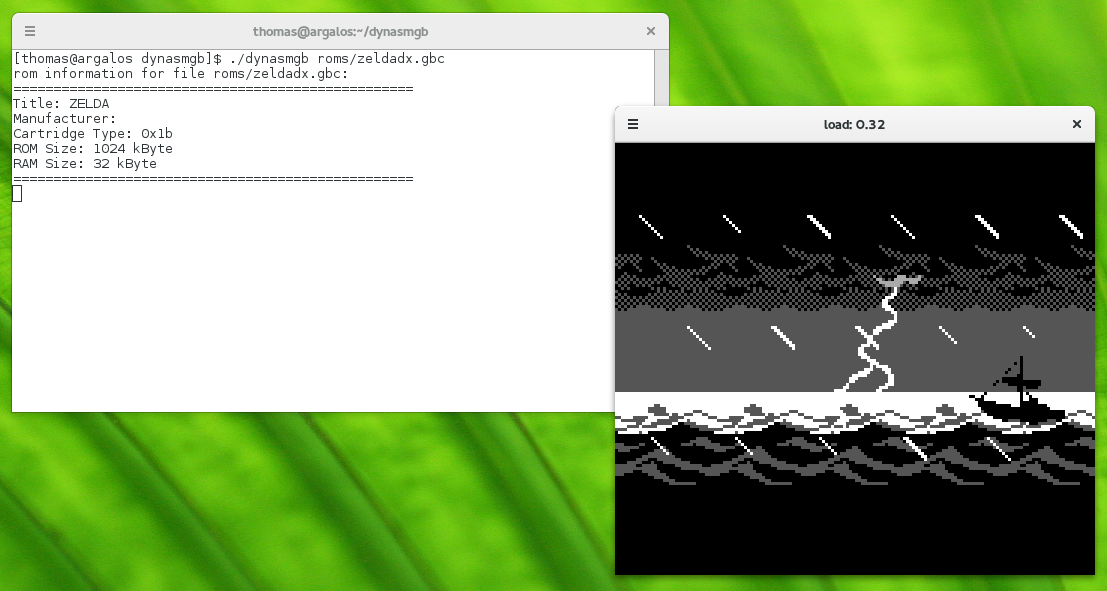
\includegraphics[width=\linewidth]{img/zelda_start}
\caption{ROM-Header Informationen für das Spiel „The Legend of Zelda -- Link's Awakening DX“.}
\label{img:zelda_start}
\end{figure}

Beim Verlassen des Spiels werden einige Statistiken zur Emulation ausgegeben: Neben der Gesamtzahl übersetzter (und gespeicherter) Blöcke wird die Startadresse des am häufigsten ausgeführten Blocks ausgegeben. Dies hilft besonders kritische Schleifen zu erkennen und entsprechende Optimierungsregeln zu schreiben. Zuletzt wird noch die Gesamtzahl ausgeführter Blöcke, die durchschnittliche Anzahl ausgeführter Blöcke pro Frame und die Anzahl angezeigter Frames angezeigt.

Falls das Spiel eine oder mehrere RAM-Bänke innerhalb der Cartridge besitzt, werden diese beim Beenden zusätzlich im Verzeichnis des Spiels als .sav-Datei gespeichert. Beim Spielstart wird der Inhalt einer solchen Datei -- falls vorhanden -- wieder in den Speicher geladen. Dies simuliert die batteriegepufferten RAM-Bänke, die in vielen Spielen zum Speichern von Spielständen verwendet werden.

\section{Debugger}

Um Emulationsfehler effektiv zu verfolgen und lokalisieren wurde eine Debuggerkonsole für das aktuell ausgeführte Spiel implementiert. Sie lässt sich durch Drücken der Taste 'd' zu einem beliebigen Zeitpunkt im Spiel, über die Startoption '-d' oder bei Erreichen eines Breakpoints aktivieren.

\begin{figure}[htbp]
\centering
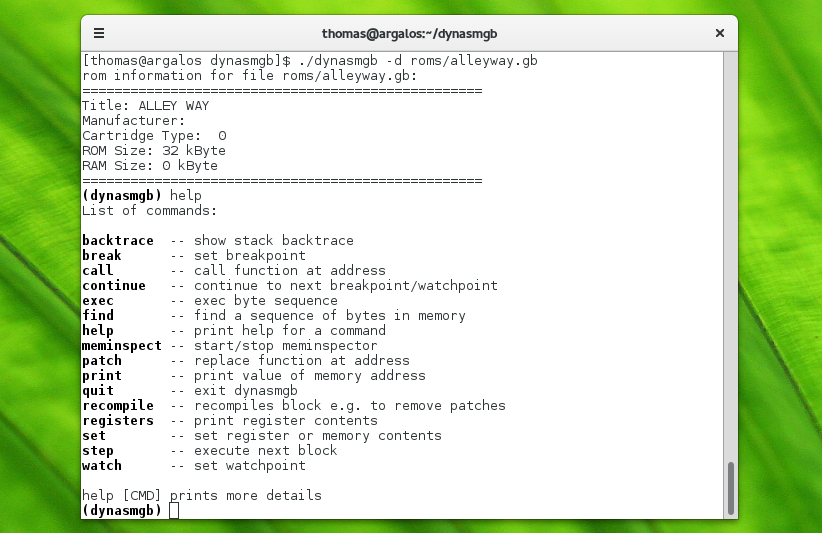
\includegraphics[width=0.8\linewidth]{img/debugger}
\caption{Debuggerkonsole.}
\label{img:debugger}
\end{figure}

Mögliche Befehle sind:
\begin{description}
\item[backtrace] Gibt den aktuellen Aufrufstack aus. Dabei wird für jeden Stackframe die Startadresse des ersten ausgeführten Blocks ausgegeben. Handelt es sich bei einem Aufruf um einen Interrupt, wird dieser rot darbestellt. Restarts werden dagegen grün dargestellt. Da sich die für den Backtrace nötigen Informationen aufgrund eines möglicherweise von Spiel zu Spiel unterschiedlichen Stacklayouts nicht oder nur schwer aus dem Speicher gewinnen lassen wird parallel zur Ausführung des Spiels bei jeder CALL oder RET Instruktion und Interrupts der Debuggerstack aktualisiert. Einige Spiele manipulieren den Aufrufstack zusätzlich durch andere Instruktionen oder kehren nicht mittels RET aus Funktionen oder Interrupts zurück -- in diesen Fällen sind die angezeigten Informationen fehlerhaft.
\item[break] Setzt einen Breakpoint für eine Startadresse eines Blocks. Bei einem Sprung auf die angegebene Adresse wird die Debuggerkonsole gestartet. Die Adresse muss dabei genau die Startadresse eines Blocks sein, Adressen innerhalb eines Blocks werden ignoriert. Derzeit wird nur ein einziger Breakpoint unterstützt und bei jedem ausgeführten Block überprüft, ob der Breakpoint erreicht wurde. Eine alternative Implementierung, die den entsprechenden Block so verändert, dass der Debugger gestartet wird und damit eine beliebige Anzahl Breakpoints ohne zusätzlichen Overhead unterstützt, ist bisher noch nicht umgesetzt aber denkbar.
\item[call] Ruft eine Funktion an einer bestimmten Speicheradresse auf. Im Unterschied zu einem „set PC \emph{address}“ kann mit einer RET-Instruktion wieder zur aktuellen Adresse zurückgekehrt werden. Ein Aufruf von „call 0x1234“ hat den gleichen Effekt wie „exec CD 34 12“, ohne dass der instruction\_count erhöht wird.
\item[continue] Verlässt die Debuggerkonsole und setzt das Spiel fort. Die Tastenkombination Strg+D hat den gleichen Effekt.
\item[exec] Übersetzt und führt eine beliebige Bytefolge aus. Die Bytes werden hexadezimal angegeben und können durch Leerzeichen oder Kommata getrennt werden. Die Bytefolge darf maximal 100 Byte lang sein. Falls die Bytefolge nicht mit einer Sprunginstruktion beendet, die den Block beendet, wird der Block stattdessen automatisch mit einer Sprunginstruktion beendet, die zur aktuellen Adresse zurückkehrt. Die Instruktionsfolge wird wie jeder andere Block, aber ohne Optimierung übersetzt. Die Ausführung beeinflusst insbesondere auch den instruction\_count und damit Timer und Interruptzeitpunkte.
\item[find] Durchsucht den gesamten Adressraum nach der angegebenen Bytefolge. Die Bytes werden hexadezimal angegeben und können durch Leerzeichen oder Kommata getrennt werden. Die Bytefolge darf maximal 20 Byte lang sein. Um die Fundstellen wird ein Kontext von jeweils 10 Byte angezeigt.
\item[help] Gibt die Abbildung~\ref{img:debugger} dargestellte Hilfe aus.
\item[meminspect] Öffnet ein zusätzliches „Memory Inspector“ sowie ein „Address Space“-Fenster. Dieses zeigt in der linken Hälfte eine Liveansicht aller schreibenden Schreibzugriffe auf die oberen 32kB des Gameboy Adressraums. In der rechten Hälfte werden unten die Gesamtzahl, sowie die aktuell in den Adressraum eingeblendeten ROM (orange) und RAM-Bänke (türkis) angezeigt. In der rechten oberen Hälfte wird eine Detailansicht der IO-Register zwischen 0xFF00 und 0xFF4F dargestellt (pink). Da nur Schreibzugriffe registriert werden, die den Speicherinhalt verändern und die Ansicht mit jedem VBLANK-Interrupt aktualisiert wird, werden Änderungen an bestimmten IO-Registern (wie zB LY) nicht angezeigt. Das „Memory-Inspector“-Fenster visualisiert die Background Tile Map, sowie die Tile Data Table für beide möglichen Startadressen (0x8000 und 0x8800). Ein weiterer Aufruf von „meminspect“ schließt das Fenster wieder.

\begin{figure}[htbp]
\centering
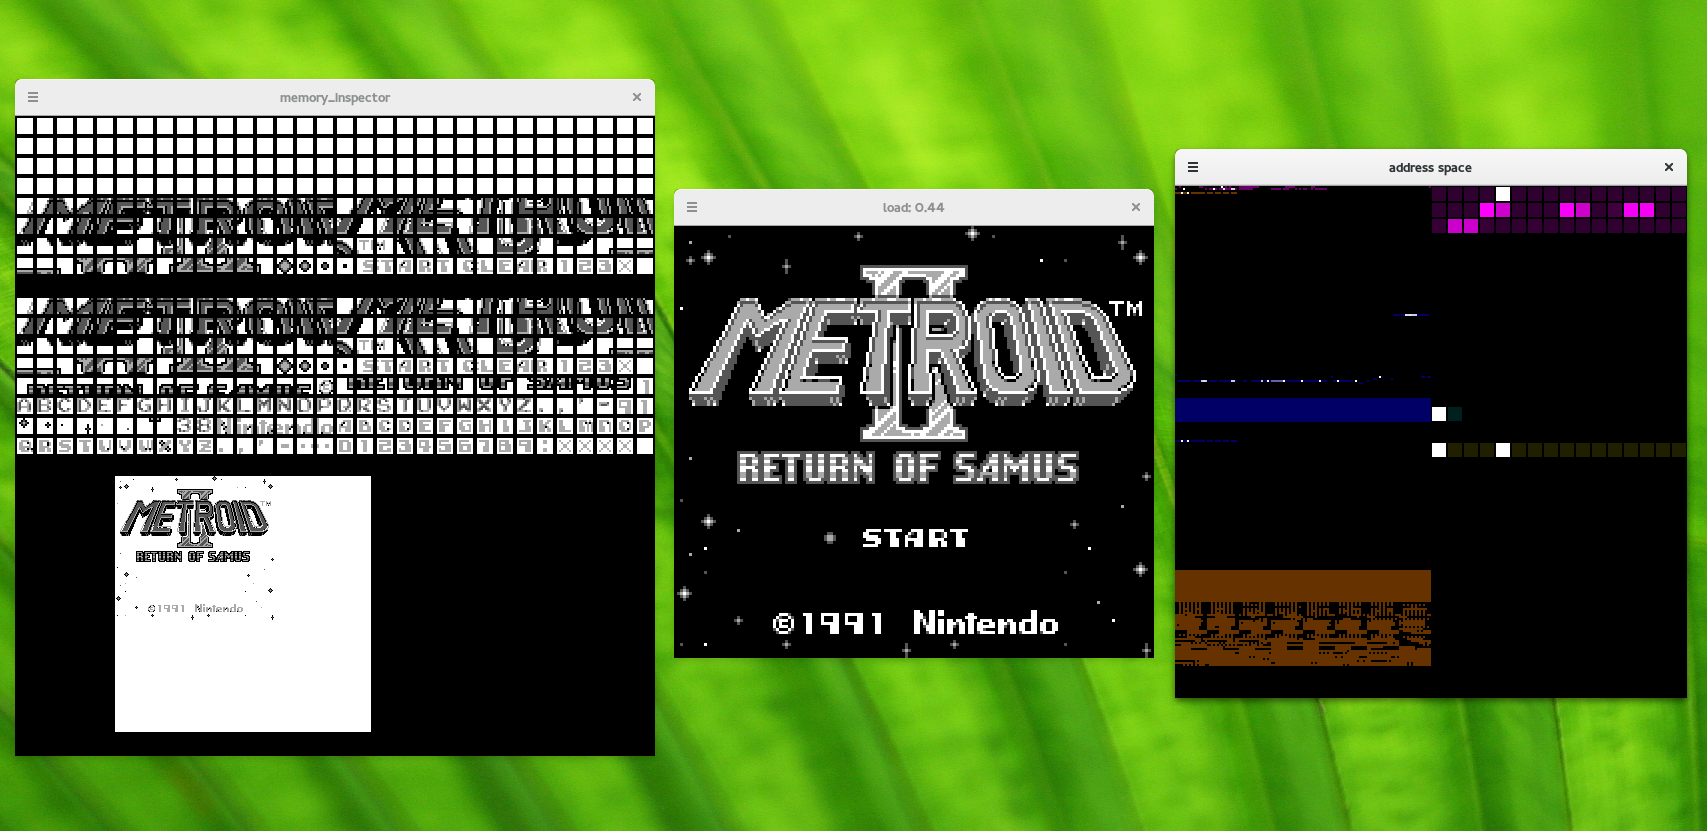
\includegraphics[width=\linewidth]{img/meminspect}
\caption{Das Spiel „Metroid II -- Return of Samus“ mit geöffnetem memory inspector.}
\label{img:meminspect}
\end{figure}

\item[patch] Ersetzt den Block mit der angegebenen Startadresse durch die angegebene Bytefolge. Es gelten die gleichen Einschränkungen wie für exec. Falls der angegebene Block nicht mit einem Sprung oder einer anderen den Block beendenden Instruktion endet wird stattdessen die aktuelle Adresse angesprungen.
\item[print] Gibt den Speicherinhalt an der (hexadezimal) angegebenen Adresse aus. Um den Wert eines Registers auszugeben kann stattdessen „registers“ verwendet werden.
\item[quit] Beendet die Emulation. Gleicher Effekt wie ESC, während das Spiel läuft.
\item[recompile] Übersetzt den Block mit der angegebenen Startadresse neu. Dabei werden keine Optimierungen angewendet. Eventuell mit „patch“ gemachte Änderungen an diesem Block werden rückgängig gemacht.
\item[registers] Gibt die Werte aller Register aus.
\item[set] Setzt den Wert eines Registers oder einer Speicheradresse. Um einen Registerwert zu ändern muss als erstes Argument das Register angegeben werden (zB „set PC 0x100“ um das Spiel zu resetten). Ist das erste Argument eine Adresse wird der entsprechende Wert in den Speicher geschrieben (zB „set 0xFFFE 0x42“). Zum Setzen der Speicheradresse wird -- wie in übersetzten Blöcken -- die Funktion write\_byte verwendet, sodass ein Schreibzugriff auf den ROM eventuell keinen Effekt hat oder zu einem Bankwechsel führt.
\item[step] Führt den nächsten Block aus. Eine leere Zeile im Debugger hat den gleichen Effekt. Derzeit wird kein Stepping über einzelne Instruktionen unterstützt.
\item[watch] Setzt einen Watchpoint für eine Speicheradresse. Ändert sich der Wert der Speicheradresse, pausiert die Emulation am Ende des Blocks und die Debuggerkonsole wird angezeigt. Derzeit kann erst am Ende des Blocks in dem der Zugriff erfolgt gestoppt und maximal ein Watchpoint gesetzt werden, da nach jedem ausgeführten Block überprüft wird, ob sich die überwachte Adresse geändert hat.
\end{description}
%unterstützte Befehle, visualisierung des Adressraums, patch, print, set, ...
\section{Kompatibilität}

Wie beschrieben implementiert dynasmgb einen Großteil der Gameboy-Architektur und Funktionalität. Der jit-Übersetzer unterstützt den kompletten Gameboy-Befehlssatz sowie wichtige Interrupts. Derzeit fehlt eine Implementierung serieller Transfers sowie des entsprechenden Interrupts.

Die Grafikemulation unterstützt alle drei Zeichenebenen (Background, Window und Sprites) nahezu vollständig. Die Reihenfolge in der die Sprites gezeichnet werden kann jedoch vom Gameboy abweichen.

Bekannte Hardwarefehler und Limitierungen des Gameboys -- unter anderem der Sprite RAM Bug, oder das Limit von 10 Sprites pro Zeile -- werden nicht emuliert. Der interne RAM wird im Unterschied zum Gameboy nicht in den Adressbereich zwischen 0xE000 und 0xFDFF gespiegelt.

Die Kompatibilität wird zusätzlich durch das möglicherweise ungenaue Timing der Interrupts und Timer-Register, sowie durch Unterschiede beim Setzen des Statusregisters eingeschränkt.

Der Emulator wurde anhand verschiedener Testroms, Beispielroms sowie komerzieller Spiele getestet.

\subsection{Blargg's GB Instruction Test}

\begin{figure}[H]
\minipage{0.45\textwidth}
  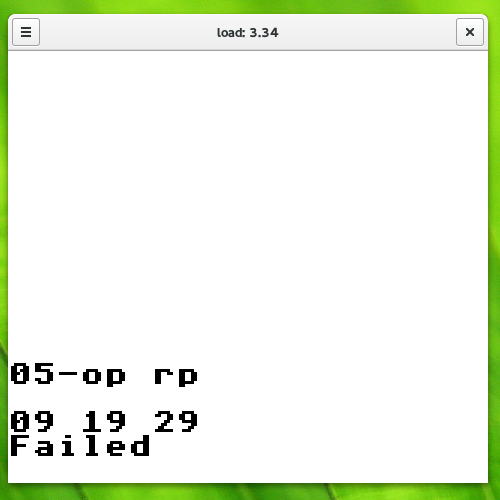
\includegraphics[width=\linewidth]{img/test_rom_fail}
\endminipage\hfill
\minipage{0.45\textwidth}
  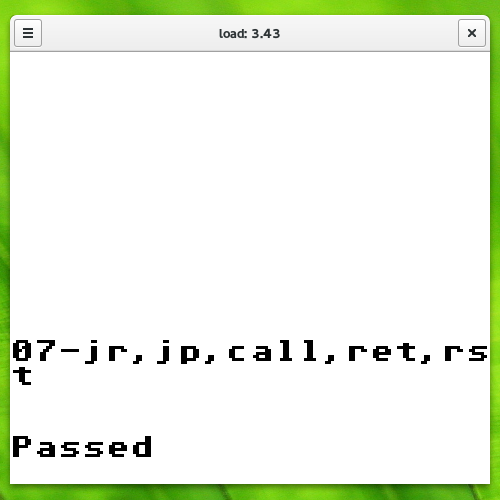
\includegraphics[width=\linewidth]{img/test_rom_pass}
\endminipage
\caption{Blagg's GB Instruction Test (Einzelne Testfälle).}
\label{img:inst_test}
\end{figure}

Blargg's GB Instruction Test \cite{test_roms} umfasst 11 Testfälle, die sämtliche Gameboyinstruktionen ausführen und die Registerinhalte nach der Ausführung mit einer CRC-Checksumme vergleichen. Dabei werden sämtliche Kombinationen von Eingabewerten und Statusflags überprüft.

\begin{figure}[H]
\centering
\begin{tabular}{l|c|c}
Testfall&Status&Erfolgreich \\
\hline
01-special&failed&4/5 \\
02-interrupts&failed&0/4 \\
03-op sp,hl&failed&3/8 \\
04-op r,imm&failed&15/16 \\
05-op rp&failed&6/9 \\
06-ld r,r&passed&64/64 \\
07-jr,jp,call,ret,rst&passed&29/29 \\
08-misc instrs&passed&19/19 \\
09-op r,r&failed&73/134 \\
10-bit ops&failed&112/168 \\
11-op a,(hl)&failed&32/51
\end{tabular}
\caption{Blagg's GB Instruction Test -- Ergebnisse.}
\label{tab:inst_test}
\end{figure}

\pagebreak
\subsection{GBDK Beispiel ROMs / PD ROMs}

Das Gameboy Developer's Kit (GBDK, \cite{gbdk}) ist eine inoffizielle Toolchain zur Entwicklung von Gameboy-Spielen in C. Es enthält einige Beispielprogramme, die zum Testen des Emulators verwendet werden können, da sie meist nur eine bestimmte Funktionalität des Gameboy ausgiebig nutzen.

\begin{figure}[H]
\centering
\minipage{0.41\textwidth}
  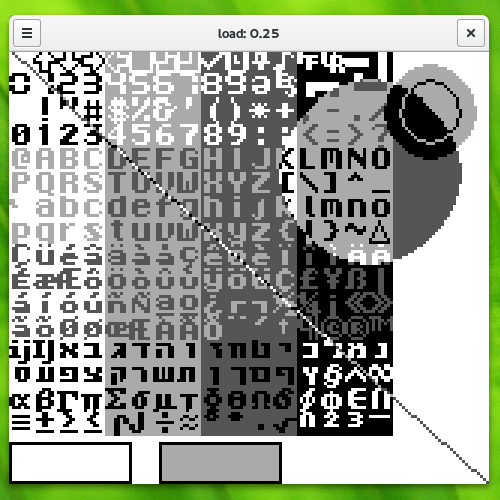
\includegraphics[width=\linewidth]{img/filltest}\vspace{0.7cm}
  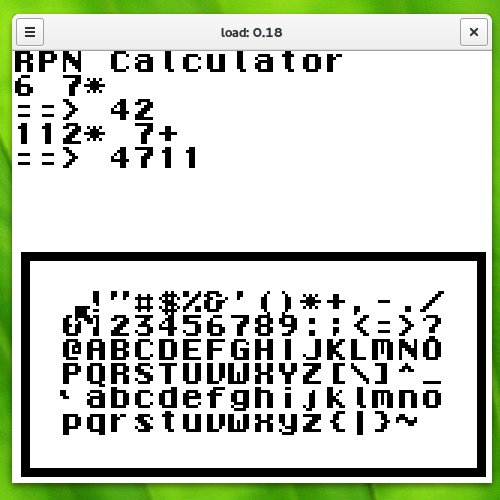
\includegraphics[width=\linewidth]{img/rpn}
\endminipage\hspace{0.7cm}
\minipage{0.41\textwidth}
  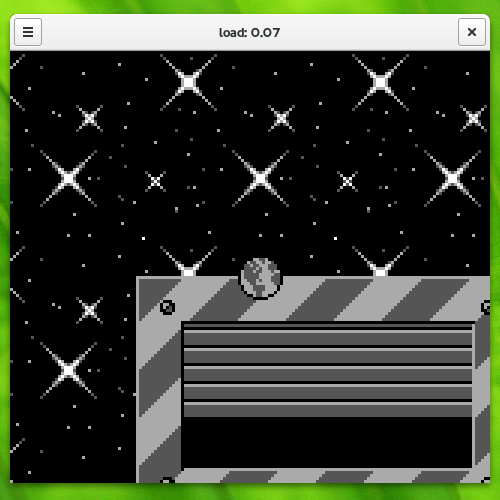
\includegraphics[width=\linewidth]{img/space}\vspace{0.7cm}
  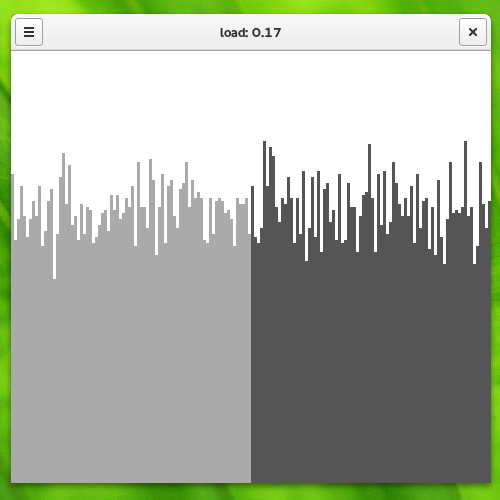
\includegraphics[width=\linewidth]{img/rand}
\endminipage
\caption{GBDK Test ROMs.}
\end{figure}

\pagebreak
\subsection{Kommerzielle Gameboy Spiele}

\begin{figure}[H]
\minipage{0.41\textwidth}
  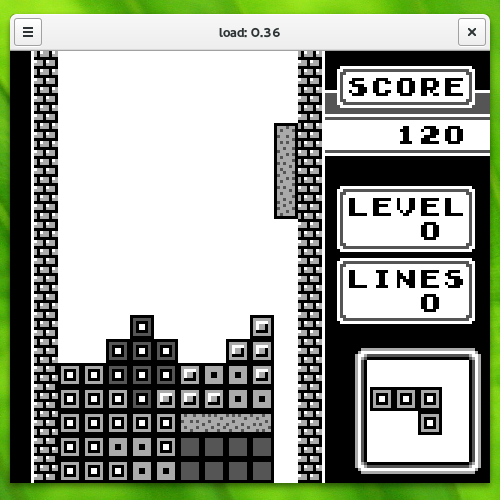
\includegraphics[width=\linewidth]{img/tetris}
\endminipage\hfill
\minipage{0.53\textwidth}
  \paragraph{Tetris}
  Tetris wurde zusammen mit dem Gameboy~Classic verkauft und ist daher das meistverkaufte Spiel für den Gameboy. Da das Spiel eine Größe von nur 32kB hat, kommt es ohne MBC aus. Es wird keine HALT-Instruktion verwendet, sodass es ein großes Optimierungspotential besitzt. Für die korrekte Emulation ist nur ein geringer Teil aller Features des Gameboy notwendig: selbst ohne Timeremulation ist das Spiel begrenzt lauffähig; der Zufallszahlengenerator um den nächsten Block auszuwählen funktioniert dann jedoch nicht.
%  \vspace{5cm}
\endminipage
\end{figure}

\begin{figure}[H]
\minipage{0.41\textwidth}
  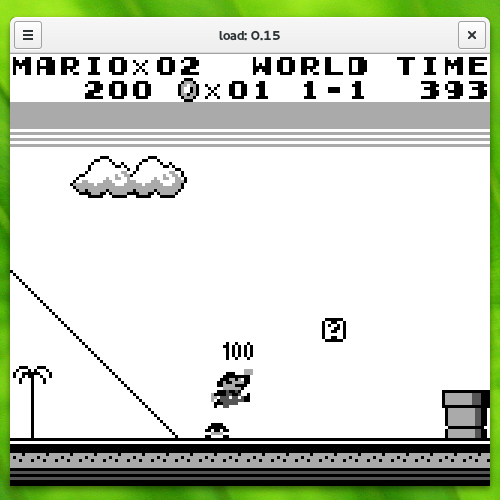
\includegraphics[width=\linewidth]{img/mario}
\endminipage\hfill
\minipage{0.53\textwidth}
  \paragraph{Super Mario World}
  Da Super Mario World eine ROM-Größe von 64kB besitzt wird ein MBC1 zur Verwaltung der vier Speicherbänke verwendet. Das Spiel nutzt fast alle graphischen Effekte bei der Spritedarstellung  und benötigt ein funktionierendes Scrollen des Hintergrunds. Eine korrekte Timer-Emulation sowie eine funktionierende DAA-Instruktion sind notwendig um die Zeitanzeige korrekt darzustellen und das Level wechseln zu können. Es wird eine größere Palette an Instruktionen verwendet als bei Tetris.
%  \vspace{5cm}
\endminipage
\end{figure}

\begin{figure}[H]
\minipage{0.41\textwidth}
  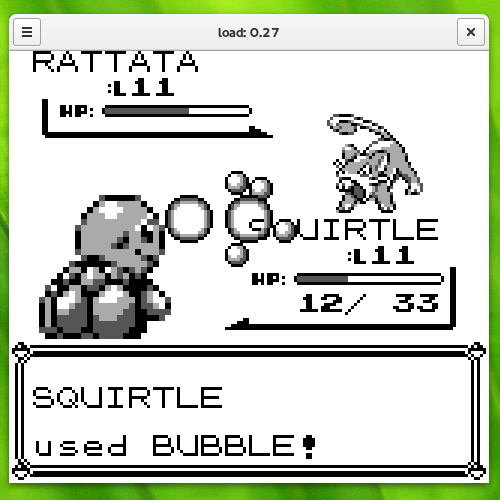
\includegraphics[width=\linewidth]{img/pokemon}
\endminipage\hfill
\minipage{0.53\textwidth}
  \paragraph{Pokémon Blaue Edition}
  Pokémon nutzt nahezu alle Funktionen des Gameboy. Zur Verwaltung des 1MB (64 Bänke) großen ROMs und der RAM-Bänke wird ein MBC5 genutzt. Um die Speicherfunktion umsetzen zu können, müssen die RAM-Bänke gespeichert werden. Da das Spiel eine Vielzahl graphischer Effekte (Wellen, invertierte Farben, etc.) für Animationen nutzt, muss sowohl ein genaues Timing, als auch eine Unterstützung sämtlicher graphischer Features existieren.
%  \vspace{5cm}
\endminipage
\end{figure}

Bei der Entwicklung wurde darauf geachtet, eine korrekte Emulation der oben genannten Spiele sicherzustellen. Es sind keine Fehler in diesen Spielen mehr bekannt, außer minimalen graphischen Fehlern in Pokémon (In manchen Scrollanimationen ist eine einzelne Zeile falsch plaziert), die wahrscheinlich durch ungenauigkeiten im Timing verursacht werden. Fast alle anderen getesteten kommerziellen Spiele funktionieren zu großen Teilen, weisen aber kleinere, das Spiel beeinflussende Fehler auf.

\begin{figure}[H]
\centering
\minipage{0.41\textwidth}
  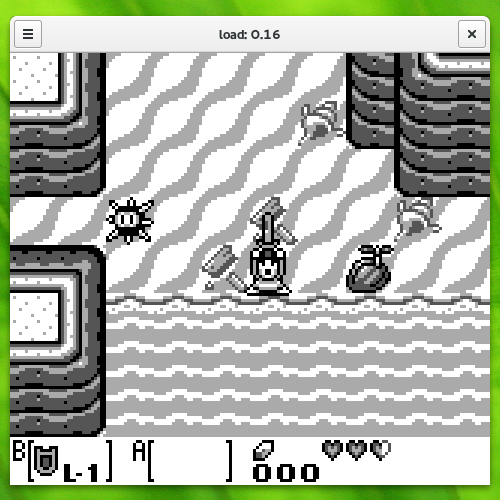
\includegraphics[width=\linewidth]{img/zelda}
  \captionsetup{labelformat=empty}
  \caption{Zelda -- Link's Awakening DX}
\endminipage\hspace{0.7cm}
\minipage{0.41\textwidth}
  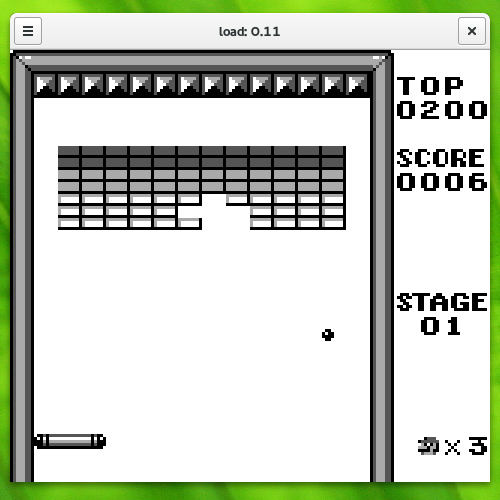
\includegraphics[width=\linewidth]{img/alleyway}
  \captionsetup{labelformat=empty}
  \caption{Alleyway}
\endminipage \vspace{0.5cm}

\minipage{0.41\textwidth}
  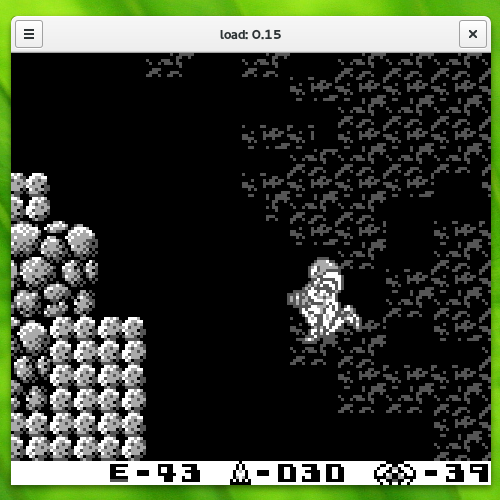
\includegraphics[width=\linewidth]{img/metroid}
  \captionsetup{labelformat=empty}
  \caption{Metroid II -- Return of Samus}
\endminipage\hspace{0.7cm}
\minipage{0.41\textwidth}
  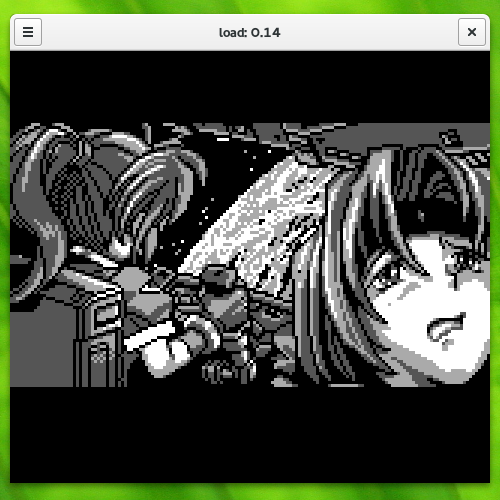
\includegraphics[width=\linewidth]{img/starocean}
  \captionsetup{labelformat=empty}
  \caption{Star Ocean -- Blue Sphere}
\endminipage

\addtocounter{figure}{-4}
\caption{Beispiele für andere, größtenteils funktionierende Spiele.}
\end{figure}

%Screenshots, bekannte Probleme
%\section{Ausblick / offene Punkte}

\pagebreak
\nocite{*}
\printbibliography

%gbc ...
\clearpage
\pagebreak
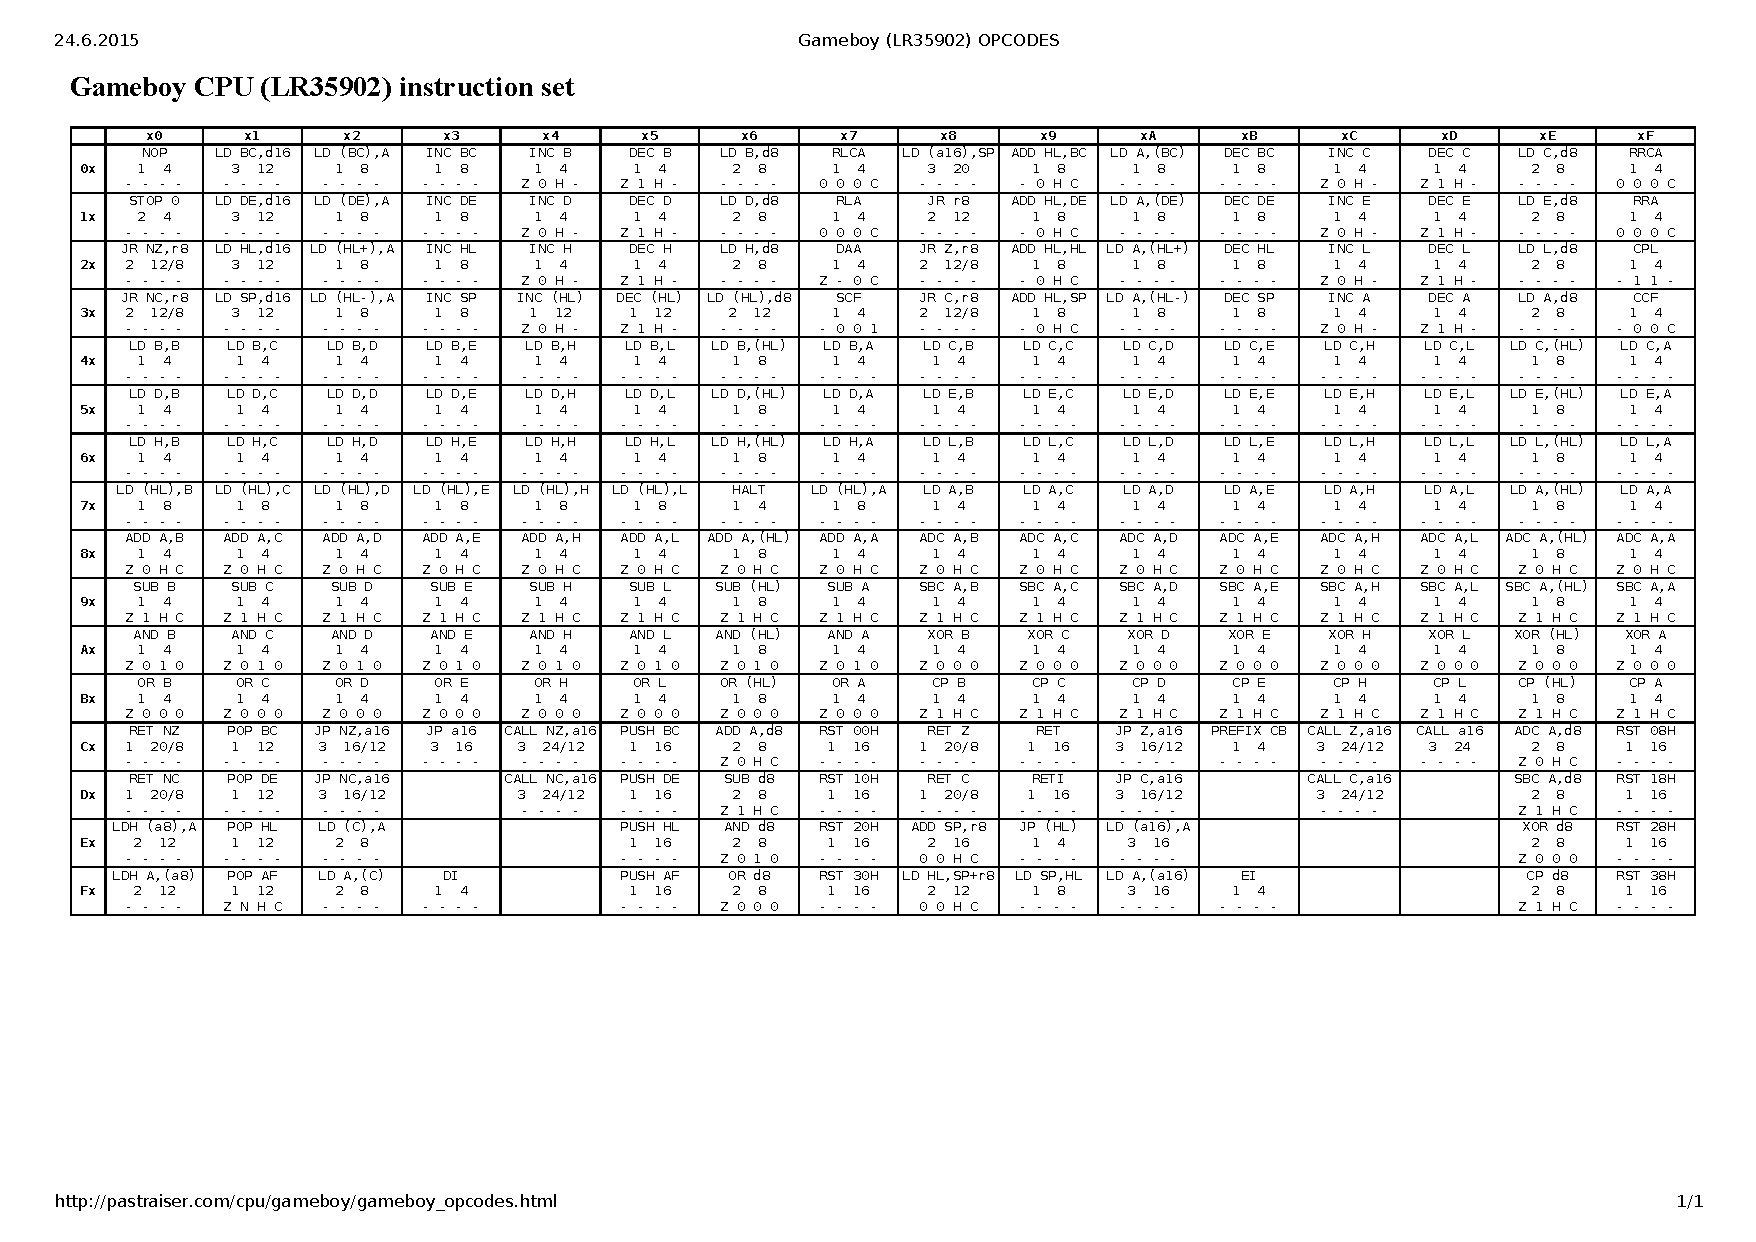
\includepdf[pages={1}, landscape]{img/OPCODES1.pdf}
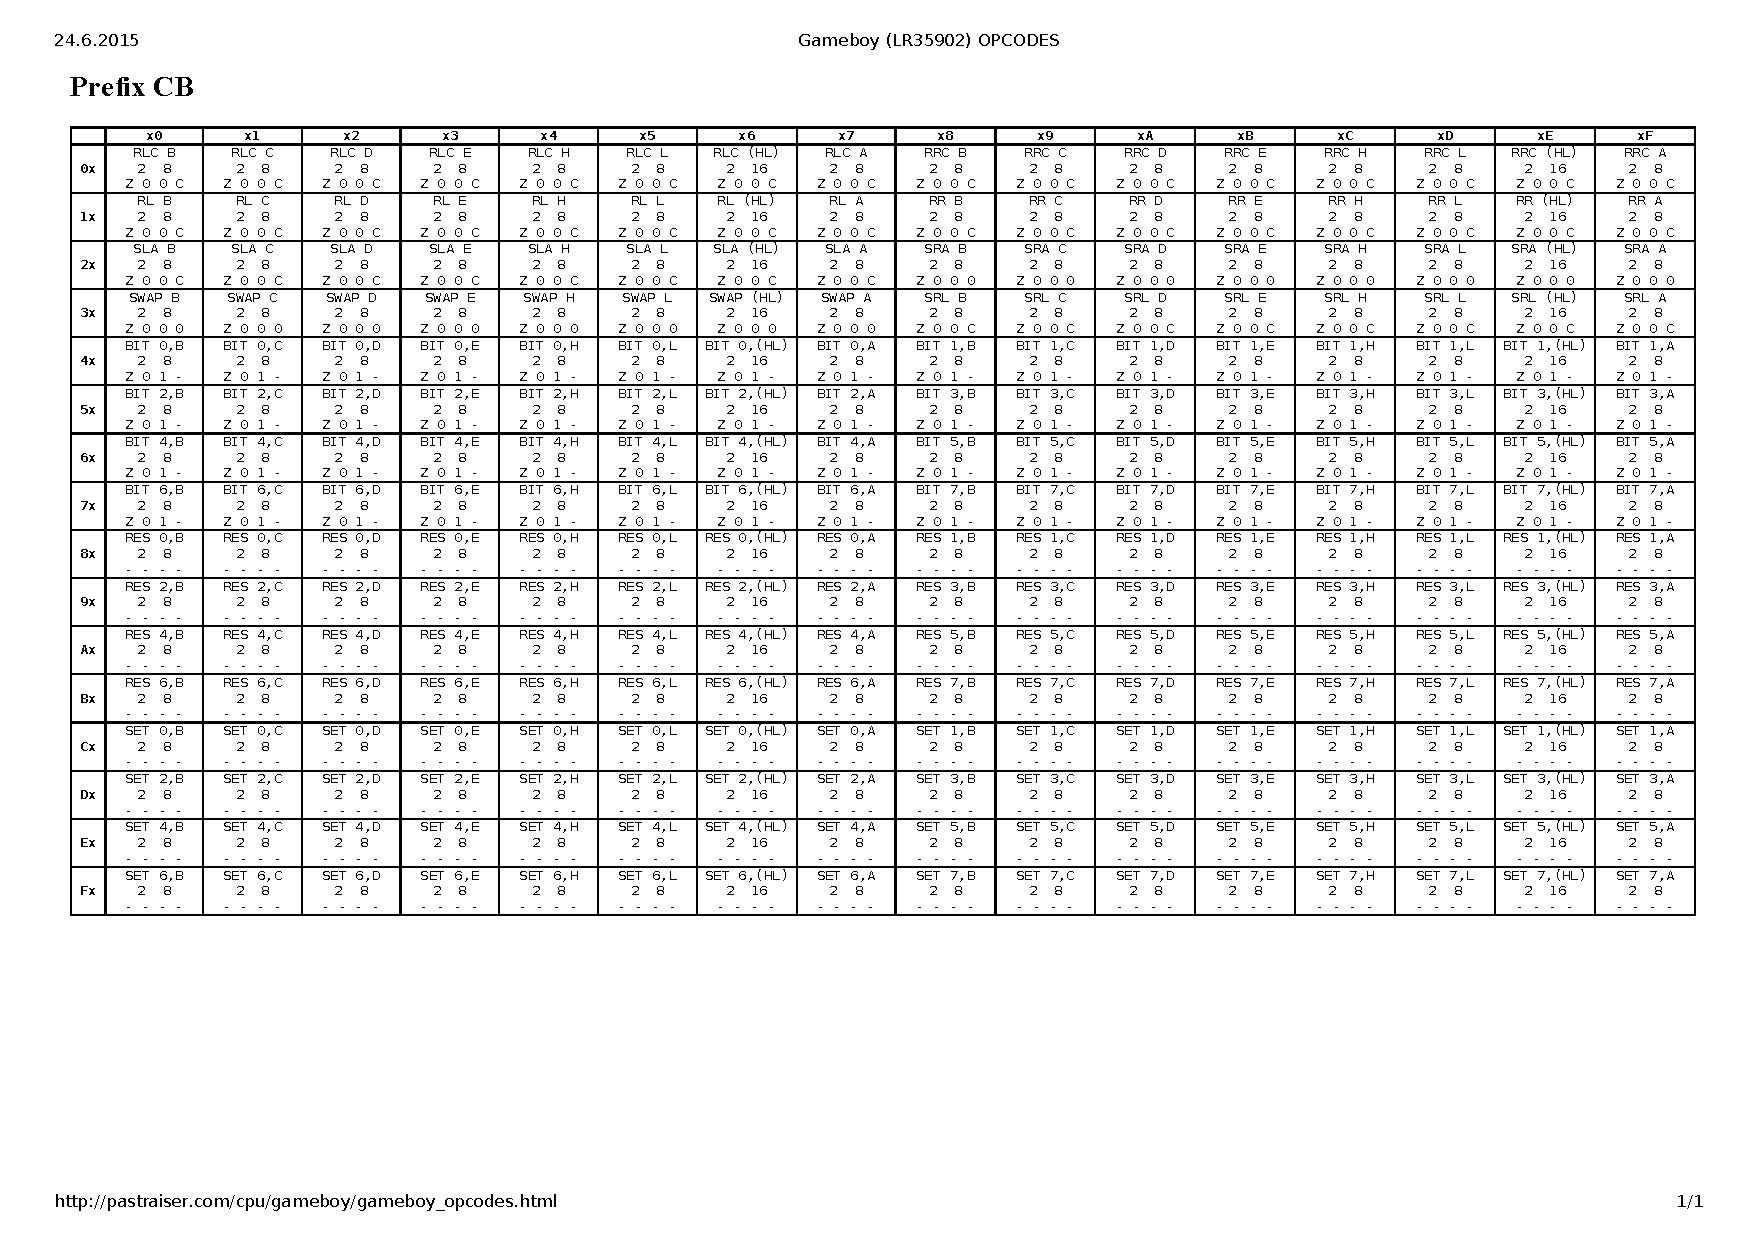
\includepdf[pages={1}, landscape]{img/OPCODES2.pdf}
\end{document}